\section{SWIM Framework and Utilities}
\label{sec:frameworkutils}
The primary software design decision in SWIM was to use scripts whenever
possible, instead of requiring the use of a particular technology. This does
mean there are multiple levels and categories encompassed by the term ``script''
but it does let us re-use existing harness, configure, and run scripts that
the different components already have available. A SWIM portal (Section
\ref{sec:portalgeneral}) has been started, but for the most part a SWIM run can
be made without using the portal at all - it is intended as a convenience and
an organizer, not as a single required entry point.

The SWIM portal-based approach is consonant with what is being
done in other national scientific collaborative efforts, and for job submission
interfaces provided by some supercomputer centers. 
An overview of portals and the tradeoffs in choosing to use them 
are in Section \ref{sec:portalgeneral}, and the particulars for the SWIM portal
are in Section \ref{sec:swimportal}.

Utilities that are near ready to be used are the job manager, the
data manager, and the event system.  Each needs more development however - in
particular the authentication and launch part of the job manager are not
yet implemented.
Some utilities, like the data manager, are accessible both through the portal
and independently via other interfaces (e.g., through Perl or ``web services''
interfaces). The job manager has two parts, one for submitting jobs via the
portal and the other for negotiating and dealing with batch managers on HPC
resources. The second one can be and is implemented via Python scripts rather
than being embedded as part of the portal itself. 


\subsection{Data Management}
\label{sec:datamanager}

% Most of the following are taken from Yu Ma's dissertation
Data management needs for \ac{swim} are complex due to the nature of
computation codes involved. Many codes have established some basic 
data staging pipelines and set up preferred I/O formats
to use data management tools like MDSplus \cite{mdsplus}. 
% need to find reference for mdsplus

% IPS doc stuff
Predefined directory structures for running simulations can be used
to keep track of data files directly. The Integrated Plasma Simulator (IPS)
Design Description document proposes the following directory layout of control 
and input files in user space. 
How to set up and populate such a simulation directory is yet to be 
discussed. 
% Include the Proposed Simulation File Tree here.
\newpage
\begin{verbatim}
IPS_run_XYZ
  |-- simulation_setup
    |-- system_config
    |-- simulation_wide_data
      |-- simulation_control_file (this is a file not a directory)
      |-- initial_plasma_state (t0) (this is a file not a directory)
      |-- machine_definition (may be empty for now)
      |-- simulation_events_waveforms 
      (scheduled events, source and control waveforms)
    |-- component_inputs
      |-- RF
        |-- RF_component (the component may need generic files)
          |-- RF_config
          |-- RF_required_list
          |-- RF_outfile_list
        |-- code_inputs (code specific files e.g. AORSA)
          |-- AORSA_required_list
          |-- AORSA_outfile_list
          |-- Standard AORSA input files  ...
      |-- FokkerPlanck
        |-- FP_component
          |-- FP_config
          |-- FP_required_list
          |-- FP_outfile_list
        |-- code_inputs (code specific input files e.g. CQL3D)
          |-- CQL3D_required_list
          |-- CQL3D_outfile_list
          |-- Standard CQL3D input files  ...
      ...		    
      |-- <other components> ...

  |-- simulation_results
    |-- history
      |-- t0 (identifier in milliseconds)
        |-- plasma_state
        |-- components
          |-- RF
          |-- Fokker Planck
          ...
          |-- <other components>
      |-- t1 (identifier in milliseconds)
        |-- plasma_state
        |-- components
          |-- RF
          |-- FokkerPlanck
          ...
          |-- <other components>
      ...		
      |-- tN ...<other time steps>
    |-- restart
      |-- t0 (identifier in milliseconds)
        |-- RF
          |-- input_files
          |-- internal_state
        |-- Fokker Planck
          |-- input_files
          |-- internal_state
        ...		    
        |-- <other components>
      |-- t1 (identifier in milliseconds)
        |-- RF
        |-- Fokker Planck
        ...
        |-- <other components> ...
      ...	
      |-- tN ...<other time steps> 
      
  |-- work
    |-- plasma_state (current plasma state tn)
    |-- RF
      |-- RF_component (the component may need generic files)
        |-- RF_config
        |-- RF_required_list
        |-- RF_outfile_list
        |-- RF_log
      |-- code_inputs (code specific input files e.g. AORSA)
        |-- AORSA_required
        |-- AORSA_outfile_list
        |-- AORSA standard input files ...
      |-- RF_component_script (?)
      |-- executable (?)
      |-- code_outputs
        |-- AORSA standard input files ...
        |-- AORSA_log
      |-- scratch
    ...	    
    |-- <other components> ...
\end{verbatim}
%
\newpage

A comprehensive predefined directory structure can be  
straightforward for locating data files of a particular simulation run, 
but could become cumbersome as the data volume grows. Supplementary
metadata management based on \ac{rdbms} techniques is beneficial in this 
case, where more sophisticated search queries and more flexible 
data storage schemas are supported. 
Additionally, new data sharing and manipulation requirements continue to 
emerge as the community framework evolves. 
For example, when different computational
components are combined to work together and interact with each other under a
distributed environment, input and output files are often shared and
duplicated among them, and likely in groups. The ability to define
an aggregate of files, and subsequently archive, locate, and retrieve them
individually or as a bundle, is beyond the scope of data management tools
already in use. Moreover, external notification mechanisms like event systems
will be deployed in the framework for different components to communicate with
each other on information like computation status and file operations,
a desired data management system should in turn interact with such an
external system for not only information exchange but also logging purpose.

For the system flexibility and extensibility, a customized data management
solution for \ac{swim} is developed under Obsidian \cite{obsidian} composable
architecture. This data manager mainly subscribes to the event channel and
responds accordingly to various data management requests described in event
messages. In addition, all related event messages are archived in
the back-end MySQL RDBMS for logging purpose, together with
Event specific metadata as defined in Table \ref{eventmd}, which are
available as query conditions for looking up particular events.
\begin{table}
\begin{center}
\begin{tabular}{|c|c|} \hline
\multicolumn{2}{|c|}{EventMD} \\ \hline \hline
EventID     &   Unique event ID \\ \hline
topic       &   Event topic as required by the event channel \\ \hline
ts          &   Timestamp of when the event is published    \\ \hline
publisher   &   User ID of who published the event      \\ \hline
component   &   Computation component ID which published the event \\ \hline
host        &   Machine host name from where the event is published \\ \hline
action      &   Progress notification or computational request  \\ \hline
message     &   Additional arbitrary user messages  \\ \hline
\end{tabular}
\caption{\label{eventmd} FSP Event Metadata}
\end{center}
\end{table}

Two initial types of data management requests have been identified as requiring
further actions from the data manager: one for archiving physical metadata of
computation component I/O files, the other for aggregating files in collections
as specified by users. Once every file of computational significance has been
recorded in the metadata database through Obsidian 
{\it Physical Location Tracker}, 
arbitrary aggregates of these files can be defined through
{\it Logical Collection Manager}, though most commonly according to job
executions of computation components.
As an example depicted in Figure \ref{fspcol}, several input and output files
are involved in two runs of the same computation. Two file collections
can then be respectively defined for those from each run,
enabling later queries to find basic metadata about all files in the same run
as a given file.
\begin{figure}
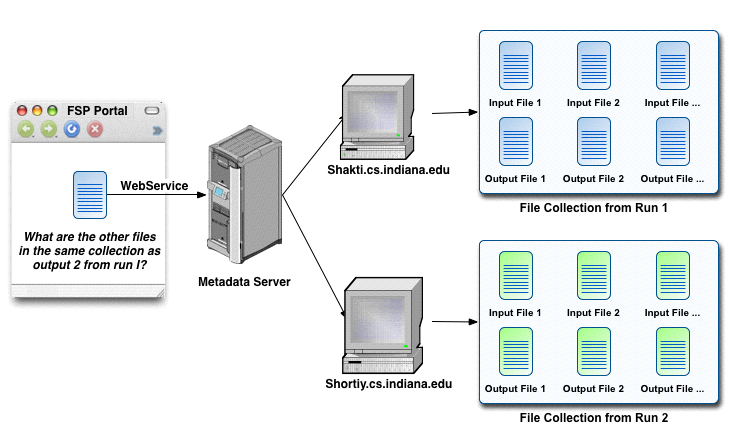
\includegraphics[scale=0.55]{file_collection.jpg}
\caption{FSP Example of Defining I/O File Aggregations}
\label{fspcol}
\end{figure}
A web service interface has been provided by the \ac{swim} data manager in
WSDL descriptions to enable interactions between the Portal and the back-end
metadata database. 
%
%\ac{swim} (like most modern scientific simulation projects) needs the ability to
%store, track, and query results. The \ac{swim} framework provides a data manager
%called Obsidian as a portlet or a standalone web service. 
However, A \ac{swim} user does not {\em have} to use the data manager and can
use another data management method like directory/file naming conventions
in place or along with it.

The data manager is used for internal information management in the portal
but end users need not deal with that.  In general three types of metadata
are defined:
        \begin{enumerator}
        \item Notifications and events published by any component or portal utility
        \item File announcements and creation. Metadata includes name, location,
              user ID of the file owner, which component created it, timestamp,
              purpose of the file, and a \ac{swim} job ID.
        \item Aggregates of files. It is convenient at times to deal with a
              collection of files such as ``all output files from a given \ac{swim}
              run'', instead of each file individually. Aggregates can be
              overlapping with a single file belonging to several at the same
              time. So ``aggregate'' does not imply the collection is a
              directory or even on the same machine.
        \end{enumerator}
        
Portal pages have been written that use the event data management to
display published events of types notification, data, and job management
dynamically. Additionally there is a portal page with a simple \ac{gui} that allows
users to enter complex queries, such as a request to view all files
belonging to user bramley created over the past week, which were used as
inputs to an RF component. If a type of query seems likely to be common
it can be added it as a predefined one, available to single users or the
whole project (via the customization capability of portals).
    
Although object storage is a more modern and flexible concept, currently
all the codes and components targeted by \ac{swim} are file-based: consuming
input and name-list files, producing output files. Files are a familiar
concept to most users. \ac{swim} provides some utilities to help coordinate,
track, and locate files.  Even without distributed computing, running
multiple codes as part of an integrated simulation requires file management
beyond what is currently done by the individual codes. The file
specification lists in {\bf SWIM\_ component\_required} and
{\bf SWIM\_component\_results}
consist of one file per line (which can be extended to allow wildcarding
later). With each file listed is an action to take: notify, save, or none.
As the names suggest, the corresponding actions are
\begin{itemize}
    \item {\em notify}: the framework will publish an event that the portal and other
          subscribers can use and act upon it - e.g., start a component that
          requires the file to exist as a prerequisite. 
    \item {\em save}: performs a notify action, and additionally signals the data
          manager to archive the file.
    \item {\em none}: no notification or action is required. The file may be listed
          because it is needed before a component can run.
\end{itemize}


\subsection{Job management}
\label{sec:jobmanager}

Job management has three parts, which are decoupled and implemented in scripts
in keeping with the SWIM overall software approach. The simplest is a user
interface for monitoring, and that is part of the SWIM portal's event
monitoring. The second part is the portal part that takes a specified component
(which at this stage are separate executables) and launches it on a specified
machine using the user's credentials for authentication. This part has been
reused from the National Fusion Grid Collaboratory, and is probably the most
onerous one for end users to get set up - but for current NFGC users SWIM will
re-use their existing grid credentials.  

The third part of job managment is the negotiation with (possibly remote) batch
management systems.
% The following was written by Sam as an outline of the batch management script
% it is basically plain text and I will make it pretty using latex later.
The batch management script {\bf batch\_mgmt\_script.py} listed in
Appendix \ref{batchscript} does this using
a Python class {\em fsp\_job}.  The class creates
{\em fsp\_job} objects which provide a common interface to PBS, SLURM, or
Unix processes. This shields users from the details of exactly how to run a
program on a specific machine.  More importantly it provides a mechanism
later on for us to submit a series of executions without having to wait
through the batch queue for each one separately. Note that this part
is {\em not} yet implemented, but the batch manager negotiator can be upgraded
to it without requiring changes to the rest of the SWIM software.

The batch negotiator includes active monitoring, checking with the batch manager
(or host OS) for the status of a job and publishing it via the event system
back to the SWIM portal - or to another event channel subscriber.

Information about the system the job is running on, what kind of job it is, the
resource requirements of the job and exact script to run are necessary for job
launch.  This information is stored in the {\bf SWIM\_config} file as a text
file of name-value pairs.  It is then parsed by the batch negotiator and run
according to the given parameters.
% We are going to have a bunch of config files. At least one for the overall
% SWIM configuration (i.e., above the individual components) and one for each
% individual component. Even I got confused about which one to use for which.
% Need to clarify that this is a per-component configuration script.

The batch negotiator allows running different codes on various systems just by
changing a few parameters in the {\bf SWIM\_config} file.  It also allows
configuring the codes to run with different versions of MPI or with different
batch managers if they are available on one machine but not another.
% The script is flexible and modular
% in that it can be extended and changed easily, then the new version is used
% everywhere without having to touch all of the different codes unnecessarily.

A detailed description of the batch negotiator, its data fields, and design
follows but most users can safely skip over them.
\begin{itemizer}
\item Data member, {\em my\_vals}, is a dictionary type that stores the
  following data:
  \begin{itemizer}
  \item  {\em batch\_mgr} : can be SLURM, or PBS, if something else is
    specified the job will be run as a regular program.  Programs are run
    differently by different batch managers.  For example, the command to
    submit a job to the queue is {\em srun} in SLURM, and {\em qsub} in PBS.
  \item  {\em num\_nodes} : this is only used when {\em batch\_mgr} is set to
    SLURM or PBS.  It is needed to specify the number of nodes needed to run
    the program at submission time.
  \item  {\em executable} : this is the name of the script file to run.  The
    script file must contain the full executable statement.  For example: ``ls''.  It is 
    recommended to use full paths.
  \item {\em jobid} : this will be set when the job is submitted.  It is used
    to monitor and cancel the job.
  \item  {\em status} : the status is set at runtime and is updated by the
    monitor function.  There are five states that are used:
    \begin{itemizer}
    \item  done : this indicates that the job no longer needs to run.  In the
      {\em \_\_init\_\_} function the state is set to done.  This corresponds to SLURM's CD
      and TO states, PBS's E state, and the UNIX command {\em ps}'s X and Z states.
    \item  trans : this indicates that the job is in some kind of transition.
      This corresponds to SLURM's CG state, PBS's T state, and the UNIX command
      {\em ps}'s T state.
    \item  failed : this indicates there was some sort of failure that occured
      while the job was running.  It only corresponds to the SLURM states F and
      NF.
    \item  waiting : this indicates that the job is waiting to use resources,
      sleeping or in the queue.  This corresponds to SLURM's PD state, PBS's Q,
      W, S and H states, and the UNIX command {\em ps}'s W, S and D states.
    \item  running : this indicates that the job is actually running.  This
      corresponds to the R state in all implemented batch managers and UNIX
      command {\em ps}.
    \end{itemizer}
  \item  {\em mpi\_job} : this allows us to do special handling for mpi jobs as
    opposed to serial jobs.
  \item  {\em Jpype} : this is the location of Jpype on the system.  Jpype is
    needed to send events to the portal.
  \item  {\em event\_channel} : this is the location of the event channel.  It
    is needed to publish events that can be picked up by the portal.
  \end{itemizer}
\item Member functions: {\em submit\_job}, {\em monitor\_job}, {\em
  remove\_from\_q}/{\em kill\_job}, {\em \_\_init\_\_}.  All the functions can
  print debugging information to standard output, in addition to, publishing events.
  \begin{itemizer}
  \item  {\em \_\_init\_\_} : reads the configuration file ({\bf
    SWIM\_config}), stores the data in {\em my\_vals}, sets the Jpype location, and
    connects to the event channel.
  \item  {\em submit\_job} : submits the job to the queue or runs the job
    (if no {\em batch\_mgr} is specified).  How, where and what is run depends
    on the values in {\em
     my\_vals} that was set up in the {\em \_\_init\_\_} function.  The {\em
     job\_id} is set at this point to allow the script to monitor and cancel the job
    automatically.
  \item  {\em monitor\_job} : this function will run continuously until the job
    finishes.  It queries the batch manager or OS for the status of the job.
    The {\em job\_id} is typically used to query for the status.  An event with
    the state and CPU time used is published at regular intervals.  The
    interval can be sent in via a paramter in the framework, or the default
    will be used.
  \item  {\em remove\_from\_q}/{\em kill\_job} : these functions will remove
    the job from the queue if it has not run yet or kill the job if it is
    currently running.  If the job has finished, the function will not do
    anything.  {\em kill\_job} just calls {\em remove\_from\_q}.
  \end{itemizer}
\end{itemizer}

Table \ref{states} shows the correspondances among the states as defined by
the different tools.  ``PROCS'' simply uses Unix processes rather than a batch
manager, and SWIM is the provided batch negotiator.
  \begin{table}
    \begin{center}
      \begin{tabular}{||l|c|c|c||} \hline \hline
        {\bf SWIM}      &  {\bf SLURM}      & {\bf PBS}  & {\bf PROCS} \\ \hline \hline
		done            &  CD,TO          &  E          &  X,Z            \\  \hline
		trans           &  CG              &  T          &  T            \\ \hline
		failed          &  F,NF            &             &               \\ \hline
		waiting         &  PD              &  Q,W,S,H    &  W,S,D        \\ \hline
		running         &  R               &  R          &  R            \\ \hline \hline
      \end{tabular}
    \end{center}
    \caption{\label{states} Possible Run States for a SWIM Component}
  \end{table}
  
Three Python dictionaries translate native batch manager states
to a uniform SWIM state idenfication:
  \begin{itemizer}
  \item  SLURM\_STATES = \{``CD'':``done'', ``TO'':``done'', ``CG'':``trans'', ``F'':``failed'',
    ``NF'':``failed'', ``PD'':``waiting'', ``R'':``running''\}
  \item PROC\_STATES = \{``X'':``done'', ``Z'':``done'', ``T'':``trans'', ``W'':``waiting'',
    ``S'':``waiting'', ``D'':``waiting'', ``R'':``running''\}
  \item PBS\_STATES = \{``E'':``done'', ``T'':``trans'', ``Q'':``waiting'', ``S'':``waiting'',
    ``W'':``waiting'', ``H'':``waiting'', ``R'':``running''\}
  \end{itemizer}  




\subsection{Event channel and decoupling}
\label{sec:eventchannel}
One of the design goals is robustness of the framework facilities,
and SWIM decouples utilities as much as possible. The main mechanism is using
an ``event channel'', a daemon service running at a well-known location.
Even different portlets running within the same portal try to use the event
channel whenever possible, instead of internal portal mechanisms.

The SWIM project uses the WS-Messenger (WSMG) \cite{wsmg,wsmgpaper} web service,
developed by the Extreme Lab at Indiana University, as an
event channel. Supporting both 
the WS-Eventing and WS-Notification specifications, WSMG is a
publish-subscribe system that allows
components or portal utilities to publish notifications
about events that occur during a run of a code.  A notification
consists of a message and a topic.  To receive notifications, a
utility must subscribe to a specific topic.  This is a
many-to-many relationship, as a subscriber can subscribe to many
different topics and a publisher's notifications may be consumed
by many different subscribers.

Using a publish-subscribe event channel like WSMG allows us to
decouple the event handling from the actual running of codes.
WSMG runs on a separate ``broker'' machine and maintains a
database of current subscriptions.  Publishers send events
consisting of a message and a topic to the broker, which then
sends the events to all subscribers interested in that particular
topic.  The publisher does not need to know which, if any,
subscribers are receiving its events.

WS-Messenger is currently being used in the Linked Environments
for Atmostpheric Discovery (LEAD)\cite{lead} project to allow remote
applications to send notification messages to each other.

\begin{figure}
\centering
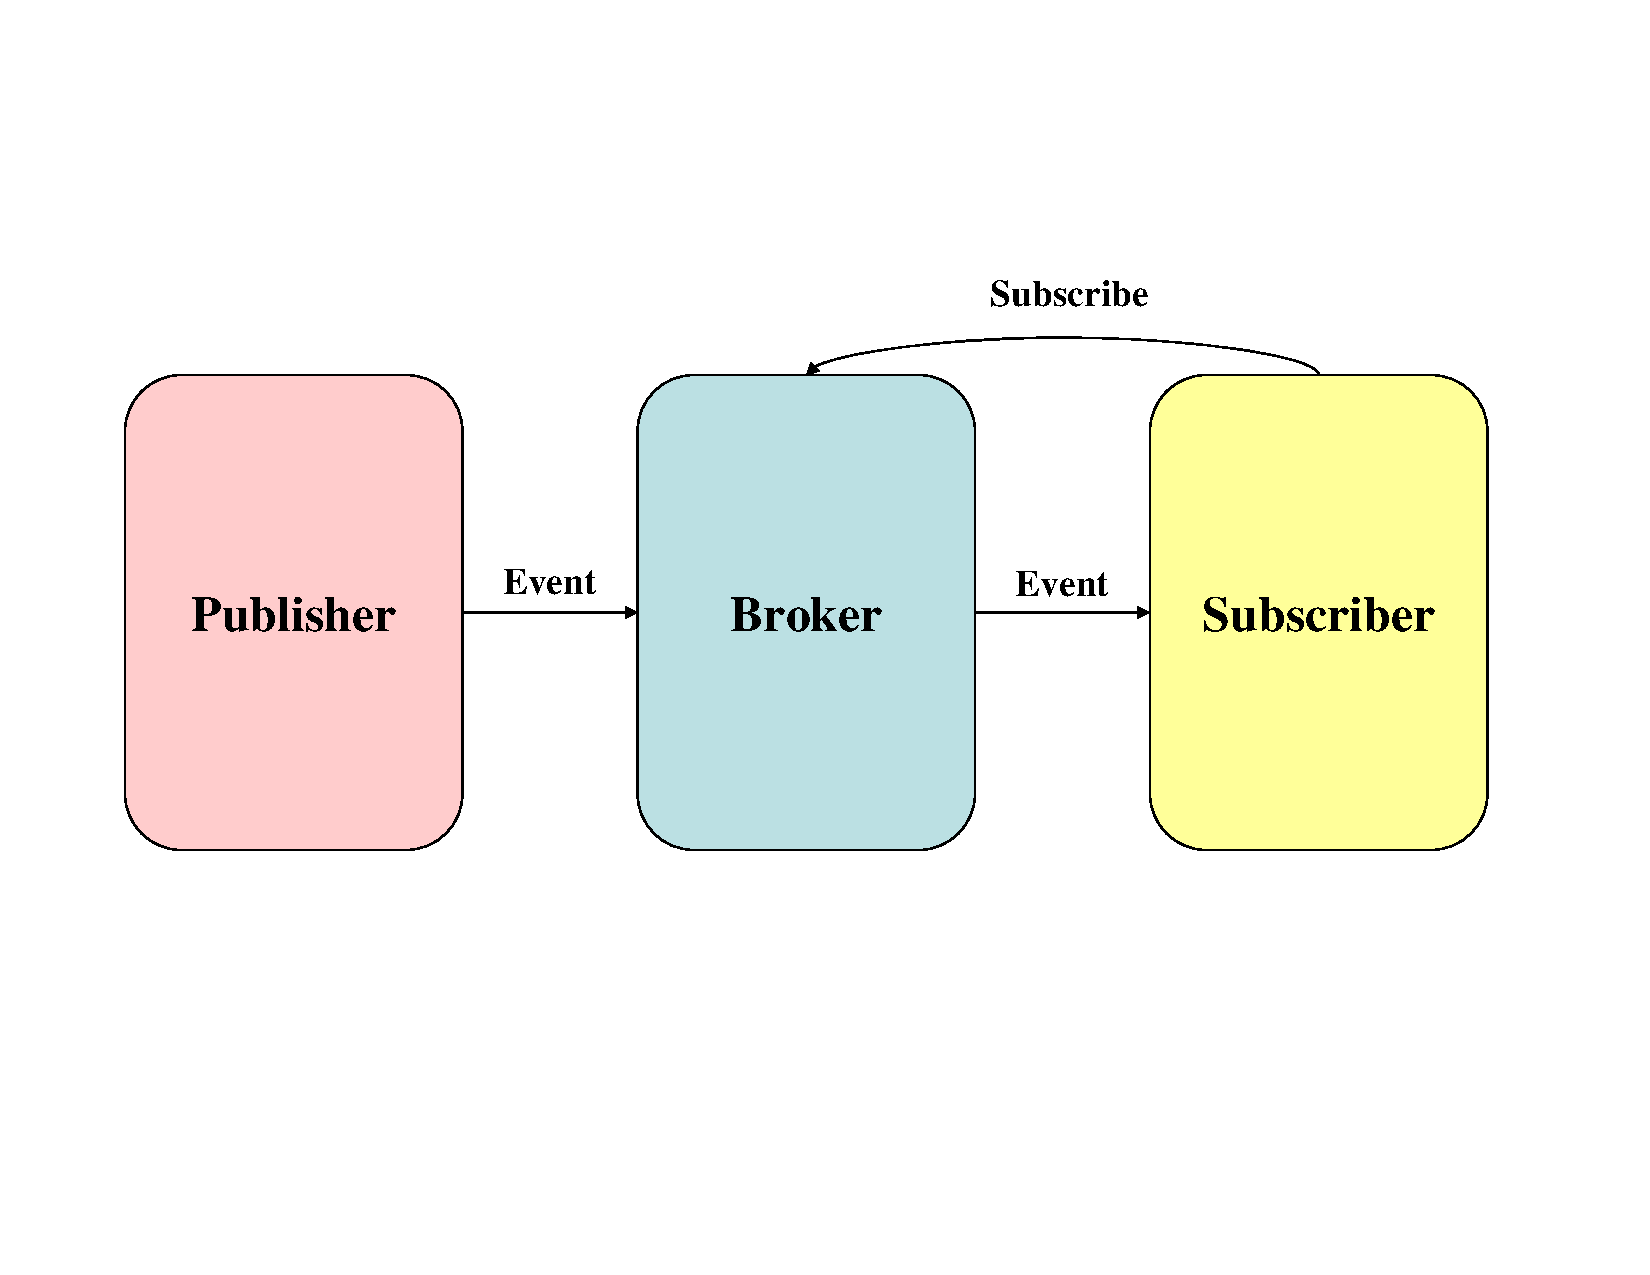
\includegraphics[width=3.0in]{eventpic}
\caption{Event Channel}
\label{eventchannelpic}
\end{figure}



\subsection{General portal ideas and terminology}
\label{sec:portalgeneral} 
The term {\em portal} originally was applied to job launch facilities provided
by the San Diego Supercomputer Center and NCSA \cite{mcat,hdf}. Portals are now used for 
job launch at remote facilities, coordination and collaboration within specific
application areas like climate \cite{climate_portal} and weather
\cite{lead} modeling, monitoring scientific
instruments \cite{cima}, and managing large scale data sets.
%can't find what reference "climate portal corresponds to

A portal is a web-based service running at some well-known location, which is
generally independent of where clients are running, managed resources are
located, or large scale scientific data sets are located. A user can launch a
set of jobs on a portal, logoff, and then reconnect later from a different
machine to check results or continue the session. A distinguishing feature of
portals is {\em customization}, meaning each user can arrange the interface for
their own interests and the server will maintain that information across
sessions for the user. Unlike most web services, that user-dependent information
is stored on the server side rather than in cookies on the user's client
machine. Customization can include what material to view, how the user interacts
with the interface, and most other aspects - but in practice most portal users
simply use the default.

Certain services that run within a portal ``container'' are called {\em
portlets}, and they have access to the information stored in the container.
Part of customization typically includes which portlets a user starts by
default. Portlets are written in Java and have to implement a
container-specified portlet interface, so that the portal can interact with
them uniformly. An end user generally should not need to write or edit portlets,
and instead new ones are added by the portal maintainers. Adding a portlet
requires some restart of the web server hosting the portal, a heavy-weight
task.

\subsection{Portal advantages and disadvantages}

Using a portal allows reuse of utilities developed across a broad range of
application areas. One of the most frequently used portlets is {\em MyProxy},
\cite{myproxy} which on logon holds a user's authentication credentials and
can present them to other (potentially remote) services on a user's behalf. 
This is necessary because as a Unix process the portal is running as some a
virtual user, and several real users may be logged in simultaneously.
{\em MyProxy} holds ``proxy certificates'' and so does not need to actually
store a user's password on the portal host.  
%can't find MyProxy reference

While {\em MyProxy} handles the problem of authentication, {\em authorization}
(determining which users can access which resources) is a separate and
more difficul problem, with several different solutions in the portal world.

Portals provide centralization, so a user's full work arena is available from
any site.  This avoids the problem of having different utilities, codes, and
working resources scattered on different machines, but does require the portal
to run on a reliable server with good network connectivity. Some portal 
implementations use techniques from commercial web servers, using load-balancing
and fail-over so that if one server host fails another can seamlessly take up
the load. SWIM is unlikely to encounter the scalability problems that some
portals have (thousands of simultaneous users) so load balancing is unlikely to
be a problem. 
Another advantage is that portal technology is being developed by several CS
research groups and companies, letting us use future upgrades and utilities
as they are developed. 

Disadvantages of using a portal approach, and how we are trying to mitigate
them, include
\begin{itemize}
  \item Authentication with remote resources is via ``grid certificates'', the
  grandchild of Globus certificates. These are X.509 certificates. SWIM will
  automatically generate the proxy certificate so that a user can login once
  per session and only have to provide a password once. But a preliminary step
  is needed to have a grid certificate created for the user.  Grid certificates
  are accepted at PPPL for the TRANSP and collaboratory projects, and are being
  used as part of ORNL's Teragrid participation.
  \item Centralization of services potentially could lead to not being able to
  do any work if the portal host is down or inaccessible. We currently have 
  fail-over capability between two machines at IU, located at Indianapolis and
  Bloomington for geographic dispersion. Both servers are on at least three
  major wide area networks (iLight, AT\&T, ESNet, Abilene). But being able to
  do fail-over among machines located under different administrative domains
  is still an open research issue, which IU is working on in the context of
  other portals. 
  \item Centralization also means the failure or loss of one utility (portlet)
    could bring down all the other portlets. We are addressing this by using
    an {\em event channel} for decoupling as much as possible (see Section
            \ref{sec:eventchannel}).
  \item Portals entail a lot of heavy-weight machinery, especially when a user
  just wants to do some
  quick debug cycling or exploratory runs. This is  mitigated partly by the
  multilevel scripting approach. The plan is to be able to run any constituent
  code as a component independently of any other, and even without access to the
  portal. Whenever a component script makes a call to a portal utility like 
  publishing a message to the event channel, if the portal is not accessible
  the script falls back to a local mechanism like writing a log file.
  The portal should be seen as a set of utilities that help compose, run,
  and diagnose SWIM runs - but it is possible to make such runs even without
  using the portal.
  \item A lot of work and effort is being put into a computer technology that
  may turn out to be a flash in the pan and outdated within a few years.
  Mitigating this is the support of portals in commercial settings by major
  companies like IBM, Sun, and lately MicroSoft, and in HPC scientific settings
  by the NSF, NIH, and DoE. The multi-level scripting approach also helps and in
  principle at least each portlet can be converted to the next generation
  container/utility technology. E.g., portlets were preceded by ``servlets'' in Java,
  and there are automatic utilities to convert a servlet to a portlet. 
  As another example,
  the data manager portlet uses an underlying MySQL database system and also
  provides scripting and ``web services'' interfaces, so running it independently
  of the portal is possible (and is done routinely in the CIMA project).
\end{itemize}
Overall, the plan is to provide the useful utilities that portals have but to
not have the project tied to that particular technology. Portals have been
around for only about 12 years now, while some control and scientific
application management scripts have been around for 40 years. 

\subsection{SWIM portal implementation}
\label{sec:swimportal} 
SWIM is using the Gridsphere portal system  \cite{gridsphere}, because it seems
to be the most widely used portal in distributed scientific computing.
%can't find gridshpere, could it be: gsi, gridftp, grid?
The implementation currently includes fiveite utilities or portlets. A standalone
{\em event channel} \cite{wsmgpaper} is used to help decouple different utilities
and the various component runs required.
    \subsubsection{Current Portlets} 
    \begin{description}
     \item {\em MyProxy}. As described earlier, this handles authentication of users:
     after logging in and providing a portal password, under the covers myproxy
     generates a ``grid certificate'' for the user and that is used to launch
     jobs and transfer data on behalf of the user. A user should never have to
     deal with or even be aware of this portlet!
     \item {\em Job Manager}.
       The portal remotely launches jobs using the batch management script.
       The launch and monitoring of the job is taken care of by the script
       automatically and uses a configuration file ({\bf SWIM\_config}) for
       specific information about how to run the code.  While the code is
       running, events are published to the portal for the user to view.
       Killing a job is also possible from this utility.
     \item {\em Data Manager}.
        This portlet is responsible for locating and moving
        files as needed for a run. It automatically generates metadata and stores
        it in a relational database, allowing users to perform queries.
        Details are in Section \ref{sec:datamanager}.
    \end{description}

\subsubsection{Event Viewer}
The SWIM portal has pages for viewing events (see Section \ref{sec:eventchannel})
as they are published.  Separate pages are provided for each type of event so
that a user does not get information overload with messages appearing on the web page.
Messages are ``pushed'' to the portal page, appearing without user action
required.
Because events are stored by the data manager, a user can also do filtering on
the messages and request, e.g., only those from a particular user or machine. 
This kind of query uses a ``pull'' approach, that is, requires a user to enter
the request or refresh the page to update it.

\subsubsection{Overall script}
The major task of the SWIM portal is to run the IPS script that specifies which
components to run, performs time looping, and makes decisions based on physics
or other criteria. Although the portal launches and runs this overall management
script (and the data manager archives it), that does not imply or require that
the script run on the portal host. Just what needs to go into this script is
specified in the IPS Design document written by Don Batchelor, and is still
evolving. The general principle is to keep individual code component run scripts
free of SWIM-specific actions and ideas, and concentrating those actions into
the overall script.

It can be edited directly on the portal page, or (a more likely usage) edited locally and
uploaded to the SWIM portal. The first case is more likely for quick debugging
and experiments since web interfaced editors generally are poor. 

